Di seguito verrà mostrato il lavoro svolto in collaborazione per avviare il progetto e, successivamente, verrà proposto ciascun contributo individuale apportato al progetto.

Nello specifico il lavoro inizialmente si è concentrato sullo studio, lo sviluppo e la scrittura di Smart Contracts per i \textit{Non-Fungible token}. Tuttavia al termine dello sviluppo e dopo un attenta ricerca si è deciso di intraprendere una strada differente e di allinearsi alla proposta di Flow, per cui determinati contratti fondamentali vengono forniti come standard in cui sono definite funzioni e risorse necessarie per lo sviluppo di sistemi basati su questo tipo di elementi. 

Di conseguenza lo \textbf{standard NFT} è stato studiato e implementato in collaborazione e verrà analizzato nella sezione \ref{sez:Flow NFT standard}, mentre quello relativo ai \textit{FungibleToken} è stato studiato e integrato al progetto per poter essere utilizzato come strumento di utilità per permettere la vendita di NFT in cambio di criptovaluta; sono state integrate anche transazioni e scripts utili per effettuare il corretto \textit{setup} dell'ambiente di test e l'implementazione \textit{FlowToken} fornita dallo standard \cite{web:FT-Standard}.

Di seguito viene mostrata una versione semplificata dell'architettura del sistema in cui si evidenziano i principali componenti utilizzati e realizzati, e le interazioni con la rete. 

\begin{figure}[H]
    \centering
    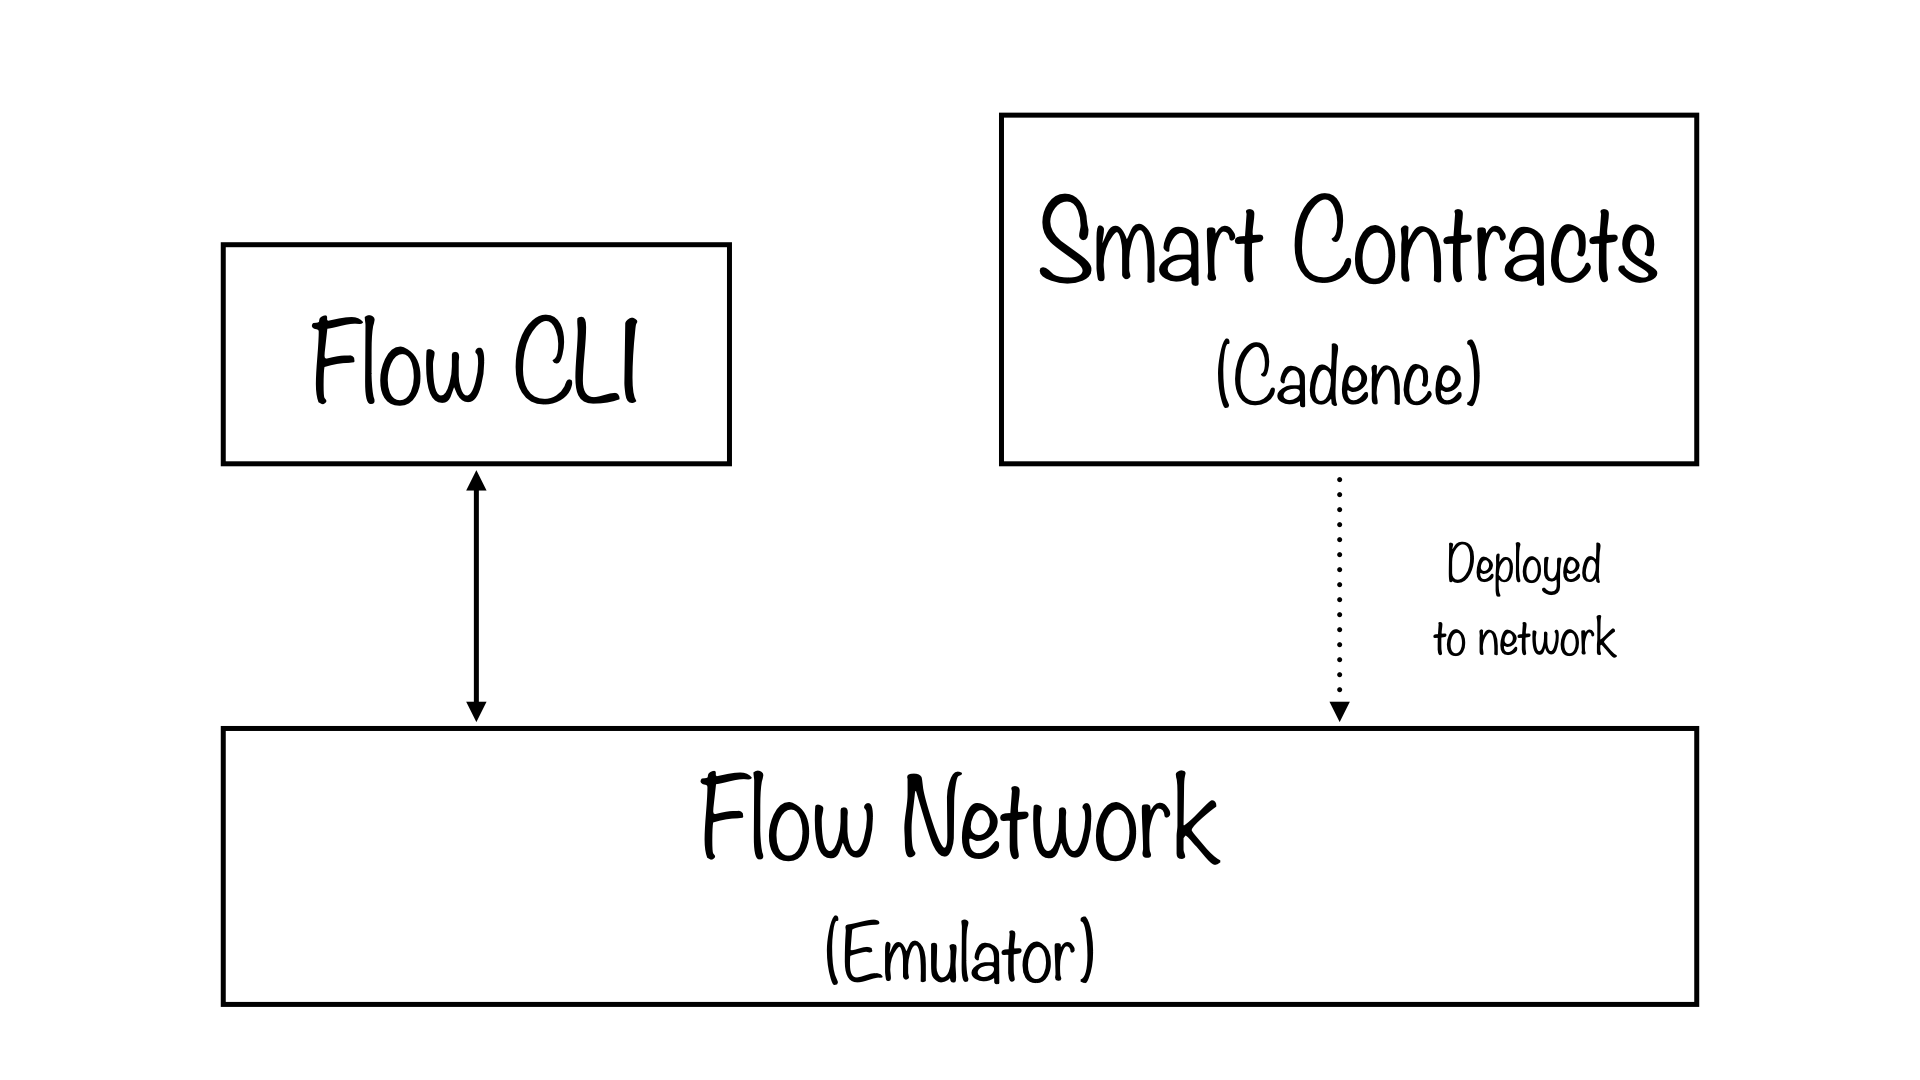
\includegraphics[width=0.8\textwidth]{img/ArchitetturaFlow.png}
    \caption{Architettura del sistema utilizzato}
    \label{fig:flowArch}
\end{figure}

Inoltre per semplificare la configurazione delle app, mette a disposizione un file chiamato \codeinline{flow.json} dal quale la CLI attinge alcune informazioni relative sia al deploy di contratti che ad indirizzi, chiavi pubbliche e aliases di determinati account, configurabili per ciascuna delle tre reti messe a disposizione da flow.

Di seguito segue il workflow comune agli use-case affrontati singolarmente:
\begin{enumerate}
    \item Si apre il terminale
    \item Viene lanciato il Flow Emulator e si crea uno snapshot del DB per mantenerne le informazioni ai successivi avvii dell'emulatore
    \item Si apre una nuova finestra del terminale (per l'esecuzione di comandi della Flow CLI)
    \item Si esegue il setup degli accounts (emulatore, Alice e Bob)
    \begin{enumerate}
        \item Ogni account inizialmente non ha FT (tranne l'emulatore)
        \item Si crea, per ogni account, una collezione vuota di NFT e se ne associa una capability 
        \item Si crea, per ogni account, la risorsa Vault (deposito per FT) e se ne associa una capability
    \end{enumerate}
    \item Si esegue il minting di due NFT da parte dell'emulatore 
    \item Gli NFT mintati sono trasferiti agli account Alice e Bob
\end{enumerate}
Si noti che queste operazioni vengono realizzate eseguendo due script, che ne contengono la logica sopra descritta: \textit{start.sh} e \textit{setup\_to\_test.sh}.

\sezione{Flow NFT standard}{capitoli/implementazioni/NFT-Standard}

\sezione{Gallo}{capitoli/implementazioni/gallo}

\sezione{Gatto}{capitoli/implementazioni/gatto}

\sezione{Moli}{capitoli/implementazioni/moli}

\sezione{Problemi riscontrati}{capitoli/implementazioni/problemi}